\documentclass[aspectratio=169,11pt]{beamer}

\usetheme{Madrid}
\usecolortheme{default}
\setbeamertemplate{navigation symbols}{}
\setbeamertemplate{footline}[frame number]

\usepackage{amsmath,amssymb}
\usepackage{graphicx}
\usepackage{tikz}
\usetikzlibrary{positioning,calc}
\usetikzlibrary{arrows.meta,decorations.pathmorphing}

\definecolor{RamRed}{RGB}{190,40,45}
\definecolor{RamBlue}{RGB}{30,90,180}
\definecolor{SoftGray}{RGB}{245,245,245}
\definecolor{DarkGray}{RGB}{70,70,70}
\definecolor{MapGreen}{RGB}{48,150,95}
\definecolor{MapGold}{RGB}{235,180,45}

\setbeamercolor{title}{fg=DarkGray}
\setbeamercolor{frametitle}{fg=white,bg=RamBlue}
\setbeamercolor{structure}{fg=RamBlue}

\tikzset{
	v/.style={circle,draw=black,fill=white,inner sep=1.8pt},
	edge/.style={draw=RamBlue,line width=1.25pt},
	topic/.style={draw=black!30,fill=SoftGray,rounded corners=5pt,inner sep=7pt,
		text width=5.8cm,minimum height=1.65cm,align=left},
}

\title[Introductory Concepts]{Introductory Concepts}
\subtitle{Section 1.1 of Harris--Hirst--Mossinghoff}
\author{Jeremy Quastel}
\date{}

\begin{document}
	
	\begin{frame}[plain]
		\centering
		\vspace{0.35cm}
		{\Huge\bfseries Introductory Concepts}\par
		\vspace{0.25cm}
		{\Large Section 1.1}\par
		\vspace{0.15cm}
		{\large Harris--Hirst--Mossinghoff, \emph{Combinatorics and Graph Theory}}\par
		
		\vspace{0.65cm}
		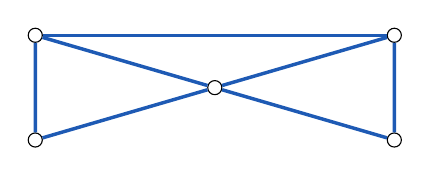
\begin{tikzpicture}[scale=0.95]
			\node[v] (a) at (-2.4,0.7) {};
			\node[v] (b) at (-2.4,-0.7) {};
			\node[v] (c) at (0,0) {};
			\node[v] (d) at (2.4,0.7) {};
			\node[v] (e) at (2.4,-0.7) {};
			\foreach \x/\y in {a/b,a/c,b/c,c/d,c/e,d/e,a/d}
			\draw[edge] (\x)--(\y);
		\end{tikzpicture}
		
		\vspace{0.3cm}
		{\large Jeremy Quastel}
	\end{frame}
	
	\begin{frame}[plain]
		\centering
		\vspace{0.15cm}
		{\Huge\bfseries Today's lecture}\par
		\vspace{0.55cm}
		
		\large
		\begin{columns}[T,onlytextwidth]
			\begin{column}{0.48\textwidth}
				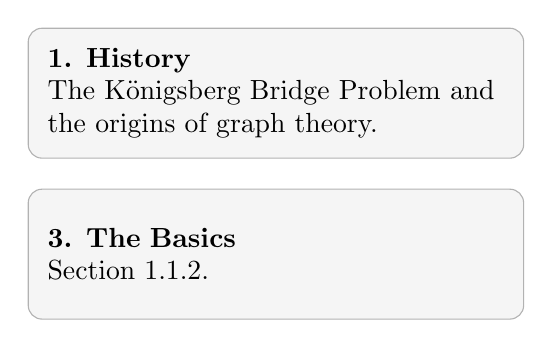
\begin{tikzpicture}
					\node[topic] (a) {\textbf{1. History}\\[-0.02cm]
						The K\"onigsberg Bridge Problem and the origins of graph theory.};
					\node[topic,below=0.38cm of a] (c) {\textbf{3. The Basics}\\[-0.02cm]
						Section 1.1.2.};
				\end{tikzpicture}
			\end{column}
			\begin{column}{0.48\textwidth}
				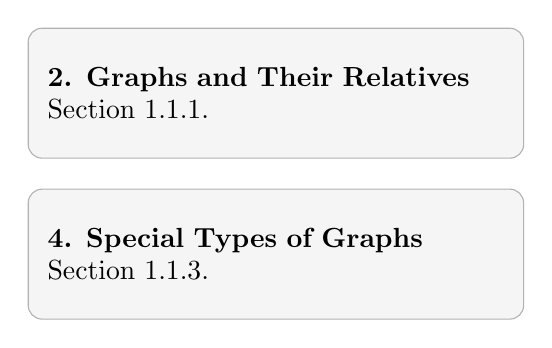
\begin{tikzpicture}
					\node[topic] (b) {\textbf{2. Graphs and Their Relatives}\\[-0.02cm]
						Section 1.1.1.};
					\node[topic,below=0.38cm of b] (d) {\textbf{4. Special Types of Graphs}\\[-0.02cm]
						Section 1.1.3.};
				\end{tikzpicture}
			\end{column}
		\end{columns}
	\end{frame}
	
	\section{History}
	
	\begin{frame}{The K\"onigsberg Bridge Problem}
		\large
		\begin{columns}[c,onlytextwidth]
			\begin{column}{0.62\textwidth}
				\centering
				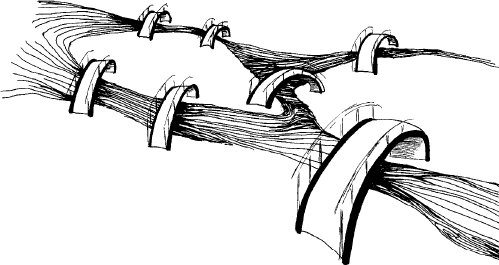
\includegraphics[width=\linewidth]{konigsberg_bridges_textbook.png}
				
				\vspace{0.12cm}
				{\scriptsize Figure 1.1: The bridges in K\"onigsberg.}
			\end{column}
			\begin{column}{0.34\textwidth}
				\normalsize
				The Pregolya River passed through the city of K\"onigsberg, where seven
				bridges connected four regions of land. The city's residents enjoyed
				walking across the bridges, but no one could find a route that crossed
				each bridge exactly once.
				
			\end{column}
		\end{columns}
		
		\vfill
		{\tiny Source: Harris, Hirst, and Mossinghoff, \emph{Combinatorics and Graph Theory}, 2nd ed., Figure 1.1.}
	\end{frame}
	
	\begin{frame}{The Four-Colour Map Conjecture}
		\large
		
		\begin{block}{Conjecture}
			Four is the maximum number of colors required to color any map where
			bordering regions are colored differently.
		\end{block}
		
		\vspace{0.28cm}
		
		\textbf{Example:} The following is a four-colouring of a graph with 8 vertices.
		
		\vspace{0.12cm}
		
		\begin{center}
			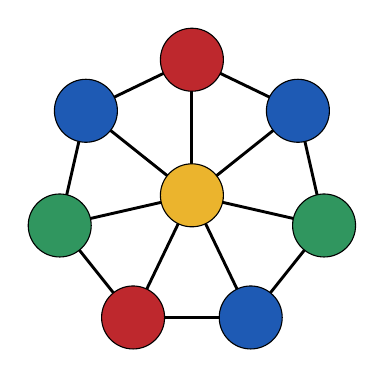
\begin{tikzpicture}[scale=0.84]
				\foreach \i/\angle in {1/90,2/141.43,3/192.86,4/244.29,
					5/295.71,6/347.14,7/38.57}
				\coordinate (p\i) at (\angle:2.05);
				
				\foreach \i/\j in {1/2,2/3,3/4,4/5,5/6,6/7,7/1}
				\draw[line width=1.05pt] (p\i)--(p\j);
				\foreach \i in {1,...,7}
				\draw[line width=1.05pt] (0,0)--(p\i);
				
				\node[circle,draw=black,fill=MapGold,minimum size=8mm] at (0,0) {};
				\node[circle,draw=black,fill=RamRed,minimum size=8mm] at (p1) {};
				\node[circle,draw=black,fill=RamBlue,minimum size=8mm] at (p2) {};
				\node[circle,draw=black,fill=MapGreen,minimum size=8mm] at (p3) {};
				\node[circle,draw=black,fill=RamRed,minimum size=8mm] at (p4) {};
				\node[circle,draw=black,fill=RamBlue,minimum size=8mm] at (p5) {};
				\node[circle,draw=black,fill=MapGreen,minimum size=8mm] at (p6) {};
				\node[circle,draw=black,fill=RamBlue,minimum size=8mm] at (p7) {};
			\end{tikzpicture}
		\end{center}
	\end{frame}
	
	\section{Introductory Concepts}
	
	\begin{frame}[plain]
		\centering
		\vfill
		{\Huge\bfseries Introductory Concepts}
		\vfill
	\end{frame}
	
	\begin{frame}{Basic Definitions}
		\normalsize
		\begin{columns}[c,onlytextwidth]
			\begin{column}{0.46\textwidth}
				\begin{block}{Graph, vertices, and edges}
					A \textbf{graph} consists of two finite sets, $V$ and $E$.
					
					\vspace{0.14cm}
					The elements of $V$ are called \textbf{vertices}.
					
					\vspace{0.14cm}
					The elements of $E$ are called \textbf{edges}. Each edge is an
					unordered pair of vertices.
				\end{block}
			\end{column}
			\begin{column}{0.50\textwidth}
				\centering
				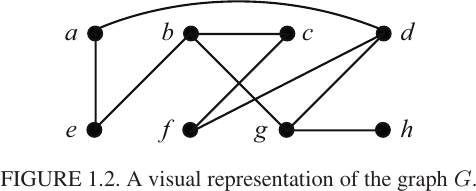
\includegraphics[width=\linewidth]{figure_1_2_graph.png}
			\end{column}
		\end{columns}
		
		\vspace{0.16cm}
		
		\begin{exampleblock}{Example}
			\small
			\[
			V=\{a,b,c,d,e,f,g,h\},
			\]
			\vspace{-0.25cm}
			\[
			E=\bigl\{\{a,d\},\{a,e\},\{b,c\},\{b,e\},\{b,g\},
			\{c,f\},\{d,f\},\{d,g\},\{g,h\}\bigr\}.
			\]
			Together, $V$ and $E$ form the graph $G$ shown in Figure 1.2.
		\end{exampleblock}
		
		\vspace{-0.02cm}
		{\tiny Source: Harris, Hirst, and Mossinghoff,
			\emph{Combinatorics and Graph Theory}, 2nd ed., Figure 1.2.}
	\end{frame}
	
	\begin{frame}{Graphs and Their Relatives}
		\large
		We can obtain similar structures by altering our definition in various ways.
		
		\vspace{0.45cm}
		\begin{columns}[c,onlytextwidth]
			\begin{column}{0.50\textwidth}
				\begin{block}{Example: A directed graph}
					By replacing our set $E$ with a set of ordered pairs of vertices, we
					obtain a \textbf{directed graph}, or \textbf{digraph}. Each edge of a
					digraph has a specific orientation.
				\end{block}
			\end{column}
			\begin{column}{0.45\textwidth}
				\centering
				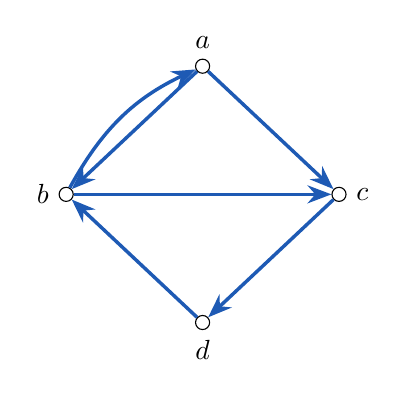
\begin{tikzpicture}[>=Stealth,scale=1.05]
					\node[v,label=above:$a$] (a) at (0,1.55) {};
					\node[v,label=left:$b$] (b) at (-1.65,0) {};
					\node[v,label=right:$c$] (c) at (1.65,0) {};
					\node[v,label=below:$d$] (d) at (0,-1.55) {};
					\draw[edge,->] (a)--(b);
					\draw[edge,->] (a)--(c);
					\draw[edge,->] (b)--(c);
					\draw[edge,->] (c)--(d);
					\draw[edge,->] (d)--(b);
					\draw[edge,->,bend left=18] (b) to (a);
				\end{tikzpicture}
				
				\vspace{0.12cm}
				{\scriptsize Figure 1.3: A digraph.}
			\end{column}
		\end{columns}
		
		\vfill
		{\tiny Source: Harris, Hirst, and Mossinghoff, \emph{Combinatorics and Graph Theory}, 2nd ed., Figure 1.3.}
	\end{frame}
	
	\begin{frame}{Next Example:}
		\large
		\begin{columns}[c,onlytextwidth]
			\begin{column}{0.50\textwidth}
				\begin{block}{A multigraph}
					If we allow repeated elements in our set of edges, technically replacing
					our set $E$ with a multiset, we obtain a \textbf{multigraph}.
				\end{block}
			\end{column}
			\begin{column}{0.45\textwidth}
				\centering
				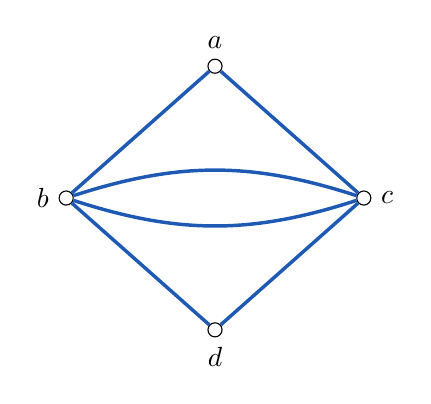
\begin{tikzpicture}[scale=1.08]
					\node[v,label=above:$a$] (a) at (0,1.55) {};
					\node[v,label=left:$b$] (b) at (-1.75,0) {};
					\node[v,label=right:$c$] (c) at (1.75,0) {};
					\node[v,label=below:$d$] (d) at (0,-1.55) {};
					\draw[edge] (a)--(b);
					\draw[edge] (a)--(c);
					\draw[edge,bend left=18] (b) to (c);
					\draw[edge,bend right=18] (b) to (c);
					\draw[edge] (b)--(d);
					\draw[edge] (c)--(d);
				\end{tikzpicture}
				
				\vspace{0.12cm}
				{\scriptsize Figure 1.4: A multigraph.}
			\end{column}
		\end{columns}
		
		\vfill
		{\tiny Source: Harris, Hirst, and Mossinghoff, \emph{Combinatorics and Graph Theory}, 2nd ed., Figure 1.4.}
	\end{frame}
	
	\begin{frame}{Next Example:}
		\large
		\begin{columns}[c,onlytextwidth]
			\begin{column}{0.50\textwidth}
				\begin{block}{A pseudograph}
					By allowing edges to connect a vertex to itself (``loops''), we obtain a
					\textbf{pseudograph}.
				\end{block}
			\end{column}
			\begin{column}{0.45\textwidth}
				\centering
				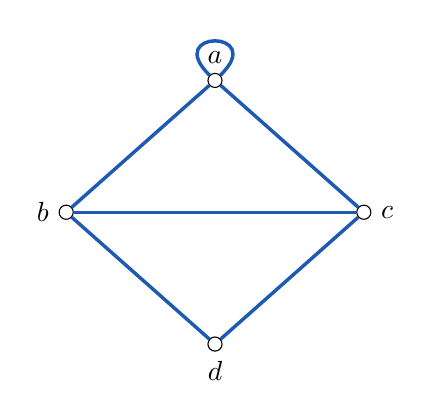
\begin{tikzpicture}[scale=1.08]
					\node[v,label=above:$a$] (a) at (0,1.55) {};
					\node[v,label=left:$b$] (b) at (-1.75,0) {};
					\node[v,label=right:$c$] (c) at (1.75,0) {};
					\node[v,label=below:$d$] (d) at (0,-1.55) {};
					\draw[edge] (a)--(b);
					\draw[edge] (a)--(c);
					\draw[edge] (b)--(c);
					\draw[edge] (b)--(d);
					\draw[edge] (c)--(d);
					\draw[edge] (a) .. controls (-0.62,2.15) and (0.62,2.15) .. (a);
				\end{tikzpicture}
				
				\vspace{0.12cm}
				{\scriptsize Figure 1.5: A pseudograph.}
			\end{column}
		\end{columns}
		
		\vfill
		{\tiny Source: Harris, Hirst, and Mossinghoff, \emph{Combinatorics and Graph Theory}, 2nd ed., Figure 1.5.}
	\end{frame}
	
	\begin{frame}{Next Example:}
		\large
		\begin{columns}[c,onlytextwidth]
			\begin{column}{0.46\textwidth}
				\begin{block}{A hypergraph}
					Allowing our edges to be arbitrary subsets of vertices, rather than just
					pairs, gives us \textbf{hypergraphs}.
				\end{block}
			\end{column}
			\begin{column}{0.50\textwidth}
				\centering
				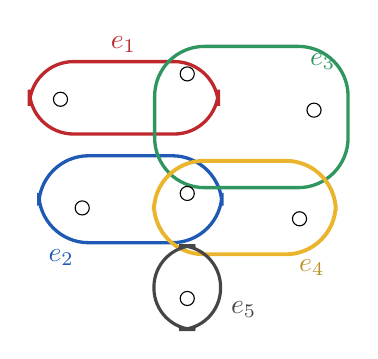
\begin{tikzpicture}[scale=0.92]
					\coordinate (a) at (-1.75,1.2);
					\coordinate (b) at (0,1.55);
					\coordinate (c) at (1.75,1.05);
					\coordinate (d) at (-1.45,-0.3);
					\coordinate (e) at (0,-0.1);
					\coordinate (f) at (1.55,-0.45);
					\coordinate (g) at (0,-1.55);
					\draw[RamRed,line width=1.2pt,rounded corners=16pt]
					(-2.18,1.72) rectangle (0.43,0.72);
					\node[RamRed] at (-0.88,1.95) {$e_1$};
					\draw[RamBlue,line width=1.2pt,rounded corners=18pt]
					(-2.05,0.42) rectangle (0.48,-0.78);
					\node[RamBlue] at (-1.74,-0.98) {$e_2$};
					\draw[MapGreen,line width=1.2pt,rounded corners=18pt]
					(-0.45,1.93) rectangle (2.22,-0.02);
					\node[MapGreen] at (1.87,1.72) {$e_3$};
					\draw[MapGold,line width=1.4pt,rounded corners=18pt]
					(-0.46,0.35) rectangle (2.05,-0.94);
					\node[MapGold!80!black] at (1.72,-1.12) {$e_4$};
					\draw[DarkGray,line width=1.15pt,rounded corners=15pt]
					(-0.46,-0.82) rectangle (0.46,-1.98);
					\node[DarkGray] at (0.78,-1.70) {$e_5$};
					\foreach \p in {a,b,c,d,e,f,g} \node[v] at (\p) {};
				\end{tikzpicture}
				
				\vspace{0.05cm}
				{\scriptsize Figure 1.6: A hypergraph with 7 vertices and 5 edges.}
			\end{column}
		\end{columns}
		
		\vfill
		{\tiny Source: Harris, Hirst, and Mossinghoff, \emph{Combinatorics and Graph Theory}, 2nd ed., Figure 1.6.}
	\end{frame}
	
	\begin{frame}{Next Example:}
		\large
		\begin{columns}[c,onlytextwidth]
			\begin{column}{0.50\textwidth}
				\begin{block}{An infinite graph}
					By allowing $V$ or $E$ to be an infinite set, we obtain \textbf{infinite
						graphs}. Infinite graphs are studied in Chapter 3.
				\end{block}
			\end{column}
			\begin{column}{0.45\textwidth}
				\centering
				
\begin{tikzpicture}[scale=1.0]
					\foreach \x in {-2.1,-1.05,0,1.05,2.1}
					\node[v] at (\x,0) {};
					\foreach \x/\y in {-2.1/-1.05,-1.05/0,0/1.05,1.05/2.1}
					\draw[edge] (\x,0)--(\y,0);
					\node at (-2.9,0) {$\cdots$};
					\node at (2.9,0) {$\cdots$};
					\draw[edge] (-2.62,0)--(-2.1,0);
					\draw[edge] (2.1,0)--(2.62,0);
				\end{tikzpicture}
				
				\vspace{0.22cm}
				{\scriptsize An infinite path.}
			\end{column}
		\end{columns}
		
		\vfill
	\end{frame}
	
	\begin{frame}{Back to Graphs}
		\normalsize
		\begin{columns}[c,onlytextwidth]
			\begin{column}{0.57\textwidth}
				\begin{block}{Vertex set}
					The vertex set of $G$, denoted by $V(G)$, is the set of its vertices.
					\[
					V(G)=\{a,b,c,d\}.
					\]
				\end{block}
				\vspace{0.15cm}
				\begin{block}{Edge set}
					The edge set of $G$, denoted by $E(G)$, is the set of its edges.
					\[
					E(G)=\{ab,bc,cd,ad\}.
					\]
					Here $ab$ is shorthand for the unordered pair $\{a,b\}$.
				\end{block}
			\end{column}
			\begin{column}{0.38\textwidth}
				\centering
				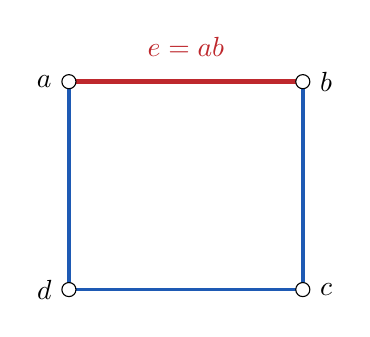
\begin{tikzpicture}[scale=1.1]
					\coordinate (a) at (-1.35,1.2);
					\coordinate (b) at (1.35,1.2);
					\coordinate (c) at (1.35,-1.2);
					\coordinate (d) at (-1.35,-1.2);
					\draw[edge] (a)--(d)--(c)--(b);
					\draw[RamRed,line width=1.8pt] (a)--node[above=5pt,text=RamRed] {$e=ab$} (b);
					\foreach \p/\pos in {a/left,b/right,c/right,d/left}
					\node[v,label=\pos:$\p$] at (\p) {};
				\end{tikzpicture}
				\par\vspace{0.25cm}
				{\large Graph $G$}
			\end{column}
		\end{columns}
		\vfill
	\end{frame}
	
	\begin{frame}{Definition: Adjacent and Incident Vertices}
		\normalsize
		\begin{columns}[c,onlytextwidth]
			\begin{column}{0.61\textwidth}
				\textbf{\color{RamBlue}Adjacent:} Vertices $u,v$ are adjacent if $uv\in E(G)$.\\
				\textit{Example:} $a$ and $b$ are adjacent.
				
				\vspace{0.22cm}
				\textbf{\color{RamBlue}Nonadjacent:} Vertices $u,v$ are nonadjacent if $uv\notin E(G)$.\\
				\textit{Example:} $a$ and $c$ are nonadjacent.
				
				\vspace{0.22cm}
				\textbf{\color{RamBlue}End vertices:} The end vertices of an edge $uv$ are $u$ and $v$.\\
				\textit{Example:} $a$ and $b$ are the end vertices of $e=ab$.
				
				\vspace{0.22cm}
				\textbf{\color{RamBlue}Incident:} A vertex is incident with an edge if it is one of its end vertices.\\
				\textit{Example:} $a$ is incident with $e$, but $c$ is not.
				
				\vspace{0.22cm}
				\textbf{\color{RamBlue}Order:} The order of $G$ is $|V(G)|$, the number of vertices.\\
				\textit{Example:} $G$ has order $4$.
			\end{column}
			\begin{column}{0.35\textwidth}
				\centering
				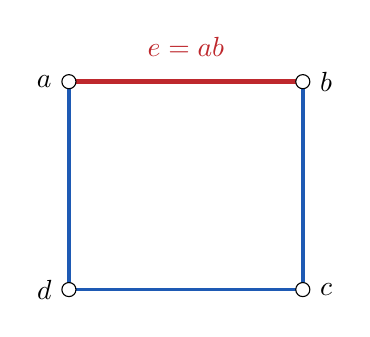
\begin{tikzpicture}[scale=1.1]
					\coordinate (a) at (-1.35,1.2);
					\coordinate (b) at (1.35,1.2);
					\coordinate (c) at (1.35,-1.2);
					\coordinate (d) at (-1.35,-1.2);
					\draw[edge] (a)--(d)--(c)--(b);
					\draw[RamRed,line width=1.8pt] (a)--node[above=5pt,text=RamRed] {$e=ab$} (b);
					\foreach \p/\pos in {a/left,b/right,c/right,d/left}
					\node[v,label=\pos:$\p$] at (\p) {};
				\end{tikzpicture}
				\par\vspace{0.25cm}
				{\large Graph $G$}
			\end{column}
		\end{columns}
		\vfill
	\end{frame}
	
	\begin{frame}{Definition: Neighborhood}
		\normalsize
		\begin{columns}[c,onlytextwidth]
			\begin{column}{0.64\textwidth}
				\textbf{\color{RamBlue}Neighborhood (open neighborhood):}\\
				$N(v)=\{x\in V(G):vx\in E(G)\}$ is the set of vertices adjacent to $v$.\\
				\textit{Example:} $N(c)=\{a,b,d\}$.
				
				\vspace{0.28cm}
				\textbf{\color{RamBlue}Closed neighborhood:}\\
				$N[v]=\{v\}\cup N(v)$.\\
				\textit{Example:} $N[c]=\{a,b,c,d\}$.
				
				\vspace{0.28cm}
				\textbf{\color{RamBlue}Neighborhood of a set:}\\
				For $S\subseteq V(G)$, $N(S)=\bigcup_{v\in S}N(v)$.\\
				\textit{Example:} For $S=\{a,d\}$,
				$N(S)=\{b,c,e\}$.
				
				\vspace{0.28cm}
				\textbf{\color{RamBlue}Closed neighborhood of a set:}\\
				$N[S]=S\cup N(S)$.\\
				\textit{Example:} $N[\{a,d\}]=\{a,b,c,d,e\}$.
			\end{column}
			\begin{column}{0.32\textwidth}
				\centering
				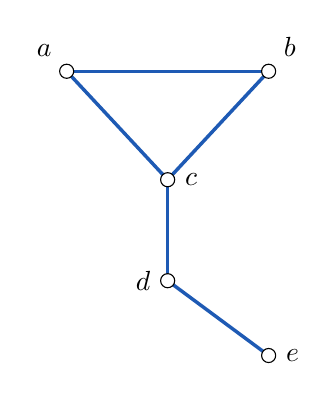
\begin{tikzpicture}[scale=0.95]
					\coordinate (a) at (-1.35,1.45);
					\coordinate (b) at (1.35,1.45);
					\coordinate (c) at (0,0);
					\coordinate (d) at (0,-1.35);
					\coordinate (e) at (1.35,-2.35);
					\foreach \x/\y in {a/b,a/c,b/c,c/d,d/e}
					\draw[edge] (\x)--(\y);
					\foreach \p/\pos in {a/above left,b/above right,c/right,d/left,e/right}
					\node[v,label=\pos:$\p$] at (\p) {};
				\end{tikzpicture}
				\par\vspace{0.2cm}
				Graph $G$
			\end{column}
		\end{columns}
	\end{frame}
	
	\begin{frame}{Definition: Degree}
		\normalsize
		\begin{columns}[c,onlytextwidth]
			\begin{column}{0.64\textwidth}
				\textbf{\color{RamBlue}Degree of a vertex:}\\
				$\deg(v)$ is the number of edges incident with $v$.\\
				For a simple graph, $\deg(v)=|N(v)|$.\\
				\textit{Example:} $\deg(c)=3$ and $\deg(e)=1$.
				
				\vspace{0.28cm}
				\textbf{\color{RamBlue}Maximum degree:}\\
				$\Delta(G)=\max\{\deg(v):v\in V(G)\}$.\\
				\textit{Example:} $\Delta(G)=3$, attained at $c$.
				
				\vspace{0.28cm}
				\textbf{\color{RamBlue}Minimum degree:}\\
				$\delta(G)=\min\{\deg(v):v\in V(G)\}$.\\
				\textit{Example:} $\delta(G)=1$, attained at $e$.
				
				\vspace{0.28cm}
				\textbf{\color{RamBlue}Degree sequence:}\\
				The list of all vertex degrees, usually in descending order.\\
				\textit{Example:} $(3,2,2,2,1)$.
			\end{column}
			\begin{column}{0.32\textwidth}
				\centering
				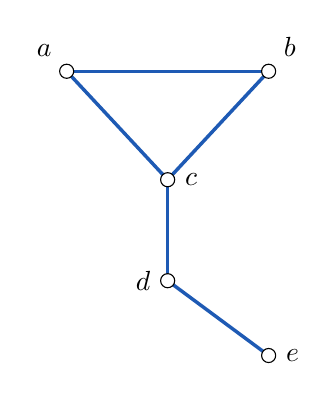
\begin{tikzpicture}[scale=0.95]
					\coordinate (a) at (-1.35,1.45);
					\coordinate (b) at (1.35,1.45);
					\coordinate (c) at (0,0);
					\coordinate (d) at (0,-1.35);
					\coordinate (e) at (1.35,-2.35);
					\foreach \x/\y in {a/b,a/c,b/c,c/d,d/e}
					\draw[edge] (\x)--(\y);
					\foreach \p/\pos in {a/above left,b/above right,c/right,d/left,e/right}
					\node[v,label=\pos:$\p$] at (\p) {};
				\end{tikzpicture}
				\par\vspace{0.2cm}
				Graph $G$
			\end{column}
		\end{columns}
	\end{frame}
	
	\begin{frame}{First Theorem of Graph Theory}
		\normalsize
		\begin{block}{Theorem}
			In a graph $G$, the sum of the vertex degrees equals twice the number of edges:
			\[
			\sum_{v\in V(G)}\deg(v)=2|E(G)|.
			\]
			Consequently, the number of vertices of odd degree is even.
		\end{block}
		
		\vspace{0.15cm}
		\begin{columns}[c,onlytextwidth]
			\begin{column}{0.61\textwidth}
				\begin{block}{Proof}
					When we sum the degrees, each edge $uv$ is counted once at $u$ and once at $v$.
					Thus every edge contributes $2$, giving the identity.
					
					\vspace{0.18cm}
					The sum is even, as is the contribution from even degrees.
					Hence the number of odd degrees is even. \hfill$\square$
				\end{block}
			\end{column}
			\begin{column}{0.35\textwidth}
				\centering
				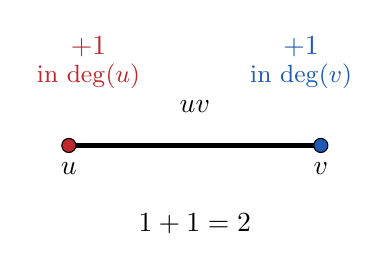
\begin{tikzpicture}[scale=1.0]
					\coordinate (u) at (-1.6,0);
					\coordinate (v) at (1.6,0);
					\draw[line width=1.5pt] (u)--node[above=8pt] {$uv$} (v);
					\node[v,fill=RamRed,label=below:$u$] at (u) {};
					\node[v,fill=RamBlue,label=below:$v$] at (v) {};
					\node[RamRed,align=center] at (-1.35,1.05) {$+1$\\[-2pt]\small in $\deg(u)$};
					\node[RamBlue,align=center] at (1.35,1.05) {$+1$\\[-2pt]\small in $\deg(v)$};
					\node at (0,-1.0) {$1+1=2$};
				\end{tikzpicture}
				\par
				{\small Each edge is counted twice.}
			\end{column}
		\end{columns}
	\end{frame}
	
	\begin{frame}{Definitions: Walks and Paths}
		\normalsize
		\begin{columns}[c,onlytextwidth]
			\begin{column}{0.64\textwidth}
				\textbf{\color{RamBlue}Walk:}\\
				A sequence $v_1,\ldots,v_k$ with $v_i v_{i+1}\in E(G)$ for $1\leq i<k$. Vertices and edges may repeat.\\
				\textit{Example:} $a,b,a,c,d,e$.
				
				\vspace{0.28cm}
				\textbf{\color{RamBlue}Path:}\\
				A walk in which all vertices are distinct.\\
				\textit{Example:} $a,b,c,d,e$.
				
				\vspace{0.28cm}
				\textbf{\color{RamBlue}End vertices:}\\
				The first and last vertices of a walk $v_1,\ldots,v_k$ are its end vertices. It is a $v_1$--$v_k$ walk.\\
				\textit{Example:} $a,b,c,d,e$ has end vertices $a$ and $e$.
				
				\vspace{0.28cm}
				\textbf{\color{RamBlue}Trail:}\\
				A walk in which all edges are distinct.\\
				\textit{Example:} $c,a,b,c,d,e$ repeats $c$, but no edge.
			\end{column}
			\begin{column}{0.32\textwidth}
				\centering
				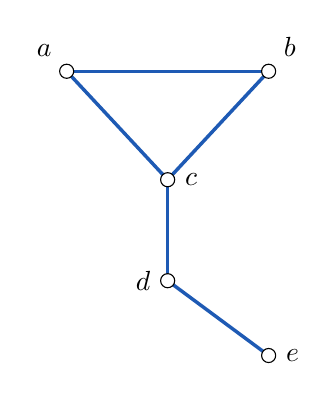
\begin{tikzpicture}[scale=0.95]
					\coordinate (a) at (-1.35,1.45);
					\coordinate (b) at (1.35,1.45);
					\coordinate (c) at (0,0);
					\coordinate (d) at (0,-1.35);
					\coordinate (e) at (1.35,-2.35);
					\foreach \x/\y in {a/b,a/c,b/c,c/d,d/e}
					\draw[edge] (\x)--(\y);
					\foreach \p/\pos in {a/above left,b/above right,c/right,d/left,e/right}
					\node[v,label=\pos:$\p$] at (\p) {};
				\end{tikzpicture}
				\par\vspace{0.2cm}
				Graph $G$
			\end{column}
		\end{columns}
	\end{frame}
	
	\begin{frame}{Definitions: Close Paths}
		\normalsize
		\begin{columns}[c,onlytextwidth]
			\begin{column}{0.64\textwidth}
				\textbf{\color{RamBlue}Closed path / Cycle:}\\
				A path $v_1,\ldots,v_k$, with $k\geq 3$, together with the edge $v_kv_1$ joining its last vertex to its first.\\
				\textit{Example:} $a,b,c,a$.
				
				\vspace{0.4cm}
				\textbf{\color{RamBlue}Closed trail / Circuit:}\\
				A trail that begins and ends at the same vertex.\\
				\textit{Example:} $c,a,b,c,d,e,c$ repeats $c$, but no edge.
				
				\vspace{0.4cm}
				\textbf{\color{RamBlue}Length of a walk:}\\
				The number of edges traversed, counting repetitions. The same definition applies to paths, trails, and cycles.\\
				\textit{Example:} $a,b,a,c,d$ has length $4$; the edge $ab$ is counted twice.
			\end{column}
			\begin{column}{0.32\textwidth}
				\centering
				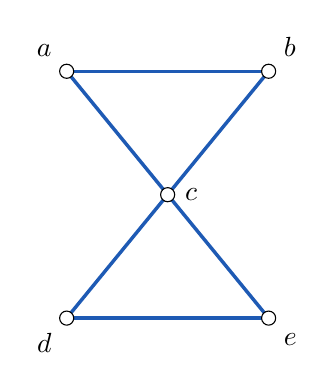
\begin{tikzpicture}[scale=0.95]
					\coordinate (a) at (-1.35,1.65);
					\coordinate (b) at (1.35,1.65);
					\coordinate (c) at (0,0);
					\coordinate (d) at (-1.35,-1.65);
					\coordinate (e) at (1.35,-1.65);
					\foreach \x/\y in {a/b,a/c,b/c,c/d,d/e,e/c}
					\draw[edge] (\x)--(\y);
					\foreach \p/\pos in {a/above left,b/above right,c/right,d/below left,e/below right}
					\node[v,label=\pos:$\p$] at (\p) {};
				\end{tikzpicture}
				\par\vspace{0.2cm}
				Graph $G$
			\end{column}
		\end{columns}
	\end{frame}
	
	\begin{frame}{Second Theorem of Graph Theory}
		\small
		\begin{columns}[c,onlytextwidth]
			\begin{column}{0.61\textwidth}
				\begin{block}{Theorem 1.2}
					In a graph $G$ with vertices $u$ and $v$, every $u$--$v$ walk contains a $u$--$v$ path.
				\end{block}
				\begin{block}{Proof}
					We induct on the length $k$ of
					$W=(u=w_0,w_1,\ldots,w_k=v)$.
					The case $k=0$ is immediate.
					
					\medskip
					If all vertices are distinct, $W$ is already a path.
					
					\medskip
					Otherwise, choose $j<r$ with $w_j=w_r$. Delete the closed portion from $w_j$ to $w_r$, leaving
					\[
					W_1:\quad w_0,\ldots,w_j,w_{r+1},\ldots,w_k.
					\]
					This shorter $u$--$v$ walk contains a $u$--$v$ path by induction. That path also lies in $W$.\hfill$\square$
				\end{block}
			\end{column}
			\begin{column}{0.35\textwidth}
				\centering
				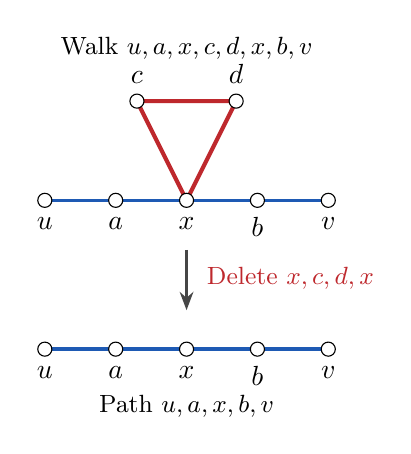
\begin{tikzpicture}[scale=0.9]
					\coordinate (u) at (-2,0);
					\coordinate (a) at (-1,0);
					\coordinate (x) at (0,0);
					\coordinate (b) at (1,0);
					\coordinate (v) at (2,0);
					\coordinate (c) at (-0.7,1.4);
					\coordinate (d) at (0.7,1.4);
					\draw[edge] (u)--(a)--(x)--(b)--(v);
					\draw[RamRed,line width=1.5pt] (x)--(c)--(d)--(x);
					\foreach \p in {u,a,x,b,v}
					\node[v,label=below:$\p$] at (\p) {};
					\node[v,label=above:$c$] at (c) {};
					\node[v,label=above:$d$] at (d) {};
					\node[font=\small] at (0,2.15) {Walk $u,a,x,c,d,x,b,v$};
					\draw[-{Stealth},thick,DarkGray] (0,-0.7)--(0,-1.55);
					\node[right,font=\small,RamRed] at (0.15,-1.1) {Delete $x,c,d,x$};
					\begin{scope}[yshift=-2.1cm]
						\draw[edge] (-2,0)--(-1,0)--(0,0)--(1,0)--(2,0);
						\foreach \p/\xx in {u/-2,a/-1,x/0,b/1,v/2}
						\node[v,label=below:$\p$] at (\xx,0) {};
						\node[font=\small] at (0,-0.8) {Path $u,a,x,b,v$};
					\end{scope}
				\end{tikzpicture}
			\end{column}
		\end{columns}
	\end{frame}
	
	\begin{frame}{Vertex and Edge Deletion}
		\normalsize
		\textbf{\color{RamBlue}Vertex deletion:}
		$G-v$ is the graph obtained by removing $v$ and every edge incident with $v$.
		
		\medskip
		\textbf{\color{RamBlue}Edge deletion:}
		$G-e$ is the graph obtained by removing only the edge $e$, keeping its end vertices.
		
		\vspace{0.35cm}
		\centering
		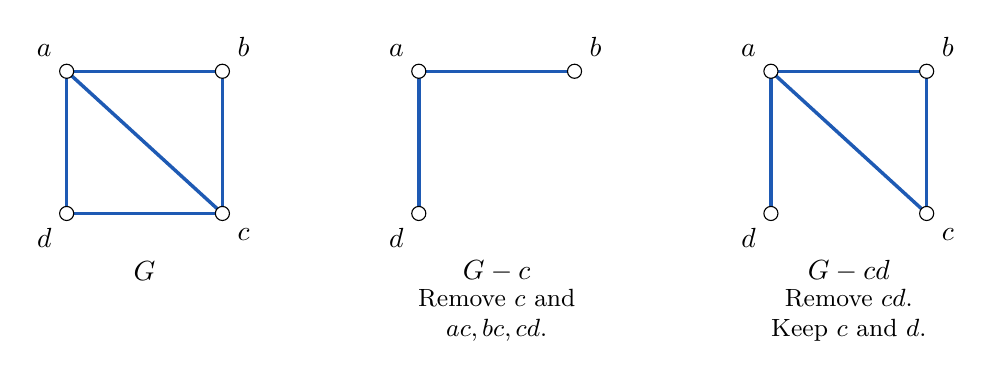
\begin{tikzpicture}[scale=0.86]
			\begin{scope}[xshift=-5.2cm]
				\coordinate (a) at (-1.15,1.05);
				\coordinate (b) at (1.15,1.05);
				\coordinate (c) at (1.15,-1.05);
				\coordinate (d) at (-1.15,-1.05);
				\foreach \x/\y in {a/b,b/c,c/d,d/a,a/c}
				\draw[edge] (\x)--(\y);
				\foreach \p/\pos in {a/above left,b/above right,c/below right,d/below left}
				\node[v,label=\pos:$\p$] at (\p) {};
				\node at (0,-1.9) {$G$};
			\end{scope}
			\begin{scope}
				\coordinate (a) at (-1.15,1.05);
				\coordinate (b) at (1.15,1.05);
				\coordinate (c) at (1.15,-1.05);
				\coordinate (d) at (-1.15,-1.05);
				\draw[edge] (a)--(b);
				\draw[edge] (a)--(d);
				\foreach \p/\pos in {a/above left,b/above right,d/below left}
				\node[v,label=\pos:$\p$] at (\p) {};
				\node at (0,-1.9) {$G-c$};
				\node[font=\small,align=center] at (0,-2.55) {Remove $c$ and\\ $ac,bc,cd$.};
			\end{scope}
			\begin{scope}[xshift=5.2cm]
				\coordinate (a) at (-1.15,1.05);
				\coordinate (b) at (1.15,1.05);
				\coordinate (c) at (1.15,-1.05);
				\coordinate (d) at (-1.15,-1.05);
				\foreach \x/\y in {a/b,b/c,d/a,a/c}
				\draw[edge] (\x)--(\y);
				\foreach \p/\pos in {a/above left,b/above right,c/below right,d/below left}
				\node[v,label=\pos:$\p$] at (\p) {};
				\node at (0,-1.9) {$G-cd$};
				\node[font=\small,align=center] at (0,-2.55) {Remove $cd$.\\Keep $c$ and $d$.};
			\end{scope}
		\end{tikzpicture}
	\end{frame}
	
	\begin{frame}{Definition: Connected Graphs}
		\normalsize
		\textbf{\color{RamBlue}Connected:} A graph is connected if every pair of vertices can be joined by a path.
		
		\medskip
		\textbf{\color{RamBlue}Disconnected:} A graph is disconnected if some pair of vertices cannot be joined by a path.
		
		\medskip
		\textbf{\color{RamBlue}Connected component:} A maximal connected subgraph, containing all vertices and edges that can be reached from any one of its vertices.
		
		\vspace{0.25cm}
		\begin{columns}[c,onlytextwidth]
			\begin{column}{0.48\textwidth}
				\centering
				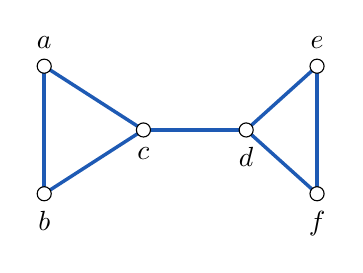
\begin{tikzpicture}[scale=0.9]
					\coordinate (a) at (-1.7,0.9);
					\coordinate (b) at (-1.7,-0.9);
					\coordinate (c) at (-0.3,0);
					\coordinate (d) at (1.15,0);
					\coordinate (e) at (2.15,0.9);
					\coordinate (f) at (2.15,-0.9);
					\foreach \x/\y in {a/b,a/c,b/c,c/d,d/e,d/f,e/f}
					\draw[edge] (\x)--(\y);
					\foreach \p/\pos in {a/above,b/below,c/below,d/below,e/above,f/below}
					\node[v,label=\pos:$\p$] at (\p) {};
				\end{tikzpicture}
				\par\vspace{0.2cm}
				\textbf{Connected}\par
				One connected component.
			\end{column}
			\begin{column}{0.48\textwidth}
				\centering
				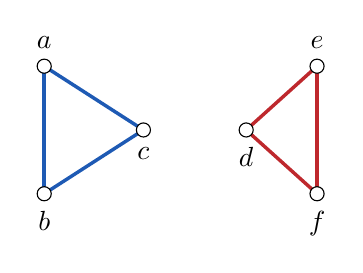
\begin{tikzpicture}[scale=0.9]
					\coordinate (a) at (-1.7,0.9);
					\coordinate (b) at (-1.7,-0.9);
					\coordinate (c) at (-0.3,0);
					\coordinate (d) at (1.15,0);
					\coordinate (e) at (2.15,0.9);
					\coordinate (f) at (2.15,-0.9);
					\foreach \x/\y in {a/b,a/c,b/c}
					\draw[edge] (\x)--(\y);
					\foreach \x/\y in {d/e,d/f,e/f}
					\draw[RamRed,line width=1.25pt] (\x)--(\y);
					\foreach \p/\pos in {a/above,b/below,c/below,d/below,e/above,f/below}
					\node[v,label=\pos:$\p$] at (\p) {};
				\end{tikzpicture}
				\par\vspace{0.2cm}
				\textbf{Disconnected}\par
				Two components: $\{a,b,c\}$ and $\{d,e,f\}$.
			\end{column}
		\end{columns}
	\end{frame}
	
	\begin{frame}{Definition: Cuts and Bridges}
		\normalsize
		\begin{columns}[c,onlytextwidth]
			\begin{column}{0.57\textwidth}
				\textbf{\color{RamBlue}Cut vertex:} A vertex $v$ is a cut vertex if $G-v$ has more connected components than $G$.
				
				\medskip
				\textit{Example:} Both $c$ and $d$ are cut vertices. Deleting either one splits $G$ into two components.
				
				\vspace{0.5cm}
				\textbf{\color{RamBlue}Bridge:} An edge $e$ is a bridge if $G-e$ has more connected components than $G$.
				
				\medskip
				\textit{Example:} The edge $cd$ is a bridge. Deleting it separates $\{a,b,c\}$ from $\{d,e,f\}$.
			\end{column}
			\begin{column}{0.39\textwidth}
				\centering
				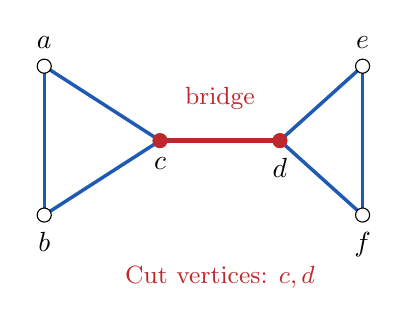
\begin{tikzpicture}[scale=1.05]
					\coordinate (a) at (-1.7,0.9);
					\coordinate (b) at (-1.7,-0.9);
					\coordinate (c) at (-0.3,0);
					\coordinate (d) at (1.15,0);
					\coordinate (e) at (2.15,0.9);
					\coordinate (f) at (2.15,-0.9);
					\foreach \x/\y in {a/b,a/c,b/c,d/e,d/f,e/f}
					\draw[edge] (\x)--(\y);
					\draw[RamRed,line width=2pt] (c)--node[above=7pt,font=\small] {bridge} (d);
					\foreach \p/\pos in {a/above,b/below,e/above,f/below}
					\node[v,label=\pos:$\p$] at (\p) {};
					\foreach \p in {c,d}
					\node[v,fill=RamRed,draw=RamRed,label=below:$\p$] at (\p) {};
					\node[RamRed,font=\small] at (0.425,-1.65) {Cut vertices: $c,d$};
				\end{tikzpicture}
				\par\vspace{0.2cm}
				Graph $G$
			\end{column}
		\end{columns}
	\end{frame}
	
	\begin{frame}{Definition: Complete Graphs}
		\normalsize
		\begin{columns}[t,onlytextwidth]
			\begin{column}{0.48\textwidth}
				\textbf{\color{RamBlue}Vertex cut set:} A proper subset $S\subsetneq V(G)$ is a vertex cut set if $G-S$ is disconnected.
				\par\vspace{0.35cm}
				\centering
				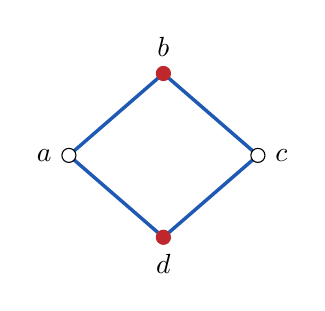
\begin{tikzpicture}[scale=0.8]
					\coordinate (a) at (-1.5,0);
					\coordinate (b) at (0,1.3);
					\coordinate (c) at (1.5,0);
					\coordinate (d) at (0,-1.3);
					\foreach \x/\y in {a/b,b/c,c/d,d/a}
					\draw[edge] (\x)--(\y);
					\foreach \p/\pos in {a/left,c/right}
					\node[v,label=\pos:$\p$] at (\p) {};
					\foreach \p/\pos in {b/above,d/below}
					\node[v,fill=RamRed,draw=RamRed,label=\pos:$\p$] at (\p) {};
				\end{tikzpicture}
				\par\vspace{0.2cm}
				$S=\{b,d\}$ is a vertex cut set.\par
				Deleting $S$ leaves isolated vertices $a,c$.
			\end{column}
			\begin{column}{0.48\textwidth}
				\textbf{\color{RamBlue}Complete graph:} A graph is complete if every pair of distinct vertices is adjacent. We write $K_n$ for the complete graph on $n$ vertices.
				\par\vspace{0.1cm}
				\centering
				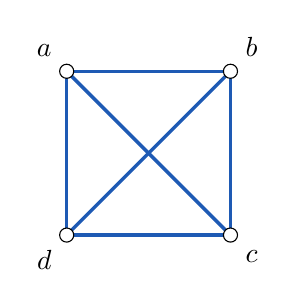
\begin{tikzpicture}[scale=0.8]
					\coordinate (a) at (-1.3,1.3);
					\coordinate (b) at (1.3,1.3);
					\coordinate (c) at (1.3,-1.3);
					\coordinate (d) at (-1.3,-1.3);
					\foreach \x/\y in {a/b,a/c,a/d,b/c,b/d,c/d}
					\draw[edge] (\x)--(\y);
					\foreach \p/\pos in {a/above left,b/above right,c/below right,d/below left}
					\node[v,label=\pos:$\p$] at (\p) {};
				\end{tikzpicture}
				\par\vspace{0.2cm}
				$K_4$: all six possible edges are present.
			\end{column}
		\end{columns}
		\vspace{0.4cm}
		\textbf{\color{RamBlue}Question:} Do complete graphs have vertex cut sets?
	\end{frame}
	
	\begin{frame}[t]{Question}
		\vspace{0.3cm}
		\begin{block}{Question}
			Let $G$ be a complete graph. Can deleting a proper subset
			$S\subsetneq V(G)$ disconnect $G$? In other words, does $G$ have a vertex cut set?
		\end{block}
	\end{frame}
	
	\begin{frame}[t]{Question}
		\vspace{0.3cm}
		\begin{block}{Question}
			Let $G$ be a complete graph. Can deleting a proper subset
			$S\subsetneq V(G)$ disconnect $G$? In other words, does $G$ have a vertex cut set?
		\end{block}
		\vspace{0.8cm}
		\begin{block}{Answer}
			No, since $G-S$ is connected for every proper subset $S\subsetneq V(G)$.
		\end{block}
	\end{frame}
	
	\begin{frame}{Definition: Connectivity}
		\small
		\begin{columns}[c,onlytextwidth]
			\begin{column}{0.61\textwidth}
				\textbf{\color{RamBlue}Connectivity:} For a non-complete graph $G$, the connectivity $\kappa(G)$ is the minimum size of a vertex cut set.
				
				\medskip
				If $G$ is disconnected, $\kappa(G)=0$. If $G$ is connected and non-complete, with $n$ vertices, then
				\[
				1\leq\kappa(G)\leq n-2.
				\]
				\textbf{\color{RamBlue}Complete graphs:} By convention, $\kappa(K_n)=n-1$. Thus, for every graph of order $n\geq 1$,
				\[
				0\leq\kappa(G)\leq n-1,
				\]
				and $\kappa(G)=n-1$ if and only if $G$ is complete.
				
				\medskip
				\textbf{\color{RamBlue}$k$-connected:} For a positive integer $k$, a graph $G$ is $k$-connected if $\kappa(G)\geq k$.
			\end{column}
			\begin{column}{0.35\textwidth}
				\centering
				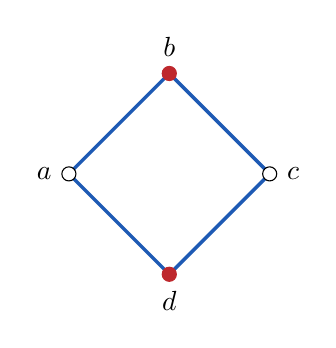
\begin{tikzpicture}[scale=0.85]
					\coordinate (a) at (-1.5,0);
					\coordinate (b) at (0,1.5);
					\coordinate (c) at (1.5,0);
					\coordinate (d) at (0,-1.5);
					\foreach \x/\y in {a/b,b/c,c/d,d/a}
					\draw[edge] (\x)--(\y);
					\foreach \p/\pos in {a/left,c/right}
					\node[v,label=\pos:$\p$] at (\p) {};
					\foreach \p/\pos in {b/above,d/below}
					\node[v,fill=RamRed,draw=RamRed,label=\pos:$\p$] at (\p) {};
				\end{tikzpicture}
				\par\vspace{0.15cm}
				\textbf{Example: $\kappa(G)=2$}\par
				\medskip
				Deleting any one vertex leaves a connected graph.\par
				\medskip
				Deleting $\{b,d\}$ disconnects it.\par
				\medskip
				So $G$ is $2$-connected.
			\end{column}
		\end{columns}
	\end{frame}
	
	\begin{frame}[t]{Prove the Following}
		\vspace{0.15cm}
		\begin{block}{Statement}
			For a graph $G$ with at least two vertices, $G$ is connected if and only if $\kappa(G)\geq 1$.
		\end{block}
	\end{frame}
	
	\begin{frame}[t]{Prove the Following}
		\vspace{0.15cm}
		\begin{block}{Statement}
			For a graph $G$ with at least two vertices, $G$ is connected if and only if $\kappa(G)\geq 1$.
		\end{block}
		\vspace{0.3cm}
		\begin{block}{If: $\kappa(G)\geq 1\ \Longrightarrow\ G$ is connected}
			If $G$ were disconnected, no vertex deletion would be needed to disconnect it, so $\kappa(G)=0$. Thus $\kappa(G)\geq 1$ implies that $G$ is connected.
		\end{block}
	\end{frame}
	
	\begin{frame}[t]{Prove the Following}
		\vspace{0.15cm}
		\begin{block}{Statement}
			For a graph $G$ with at least two vertices, $G$ is connected if and only if $\kappa(G)\geq 1$.
		\end{block}
		\vspace{0.3cm}
		\begin{block}{If: $\kappa(G)\geq 1\ \Longrightarrow\ G$ is connected}
			If $G$ were disconnected, no vertex deletion would be needed to disconnect it, so $\kappa(G)=0$. Thus $\kappa(G)\geq 1$ implies that $G$ is connected.
		\end{block}
		\vspace{0.3cm}
		\begin{block}{Only if: $G$ is connected $\ \Longrightarrow\ \kappa(G)\geq 1$}
			If $G$ is connected and non-complete, deleting no vertices leaves it connected. Every vertex cut set therefore has at least one vertex, so $\kappa(G)\geq 1$.
			
			\medskip
			If $G=K_n$, then $\kappa(G)=n-1\geq 1$ because $n\geq 2$.
		\end{block}
	\end{frame}
	
	\begin{frame}[t]{Prove the Following}
		\small
		\vspace{0.15cm}
		\begin{block}{Statement}
			For a graph $G$ with at least three vertices, $\kappa(G)\geq 2$ if and only if $G$ is connected and has no cut vertices.
		\end{block}
	\end{frame}
	
	\begin{frame}{Other Things You Can Prove}
		\normalsize
		\begin{enumerate}
			\item[(ii)] For a graph $G$ with at least three vertices, $\kappa(G)\geq 2$ if and only if $G$ is connected and has no cut vertices.
			
			\vspace{0.65cm}
			\item[(iii)] Every $2$-connected graph contains at least one cycle.
			
			\vspace{0.65cm}
			\item[(iv)] For every graph $G$, $\kappa(G)\leq\delta(G)$.
		\end{enumerate}
	\end{frame}
	
	\begin{frame}{Special Types of Graphs}
		\begin{block}{Complete graphs}
			The complete graph $K_n$ has $n$ vertices, with an edge between every pair of distinct vertices.
		\end{block}
		\vspace{0.2cm}\centering
		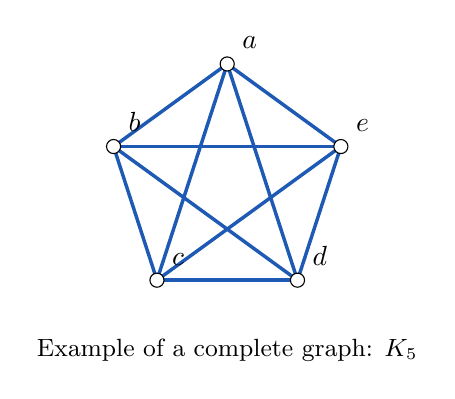
\begin{tikzpicture}[scale=0.92]
			\begin{scope}[xshift=0cm]
				\coordinate (a) at (0.0,1.65);
				\coordinate (b) at (-1.569,0.51);
				\coordinate (c) at (-0.97,-1.335);
				\coordinate (d) at (0.97,-1.335);
				\coordinate (e) at (1.569,0.51);
				\draw[edge] (a)--(b);
				\draw[edge] (a)--(c);
				\draw[edge] (a)--(d);
				\draw[edge] (a)--(e);
				\draw[edge] (b)--(c);
				\draw[edge] (b)--(d);
				\draw[edge] (b)--(e);
				\draw[edge] (c)--(d);
				\draw[edge] (c)--(e);
				\draw[edge] (d)--(e);
				\node[v,label=above right:$a$] at (a) {};
				\node[v,label=above right:$b$] at (b) {};
				\node[v,label=above right:$c$] at (c) {};
				\node[v,label=above right:$d$] at (d) {};
				\node[v,label=above right:$e$] at (e) {};
				\node[font=\small,align=center] at (0,-2.3) {Example of a complete graph: $K_5$};
			\end{scope}
		\end{tikzpicture}
	\end{frame}
	
	\begin{frame}{Special Types of Graphs}
		\begin{block}{Empty graphs}
			The empty graph $E_n$ has $n$ vertices and no edges. Its edge set is $\varnothing$.
		\end{block}
		\vspace{0.2cm}\centering
		\begin{tikzpicture}[scale=0.92]
			\begin{scope}[xshift=0cm]
				\coordinate (a) at (0.0,1.65);
				\coordinate (b) at (-1.429,0.825);
				\coordinate (c) at (-1.429,-0.825);
				\coordinate (d) at (-0.0,-1.65);
				\coordinate (e) at (1.429,-0.825);
				\coordinate (f) at (1.429,0.825);
				\node[v,label=above right:$a$] at (a) {};
				\node[v,label=above right:$b$] at (b) {};
				\node[v,label=above right:$c$] at (c) {};
				\node[v,label=above right:$d$] at (d) {};
				\node[v,label=above right:$e$] at (e) {};
				\node[v,label=above right:$f$] at (f) {};
				\node[font=\small,align=center] at (0,-2.3) {Example of an empty graph: $E_6$};
			\end{scope}
		\end{tikzpicture}
	\end{frame}
	
	\begin{frame}{Special Types of Graphs}
		\begin{block}{Complements}
			The complement $\overline{G}$ has the same vertices as $G$. Two distinct vertices are adjacent in $\overline{G}$ exactly when they are not adjacent in $G$.
		\end{block}
		\vspace{0.2cm}\centering
		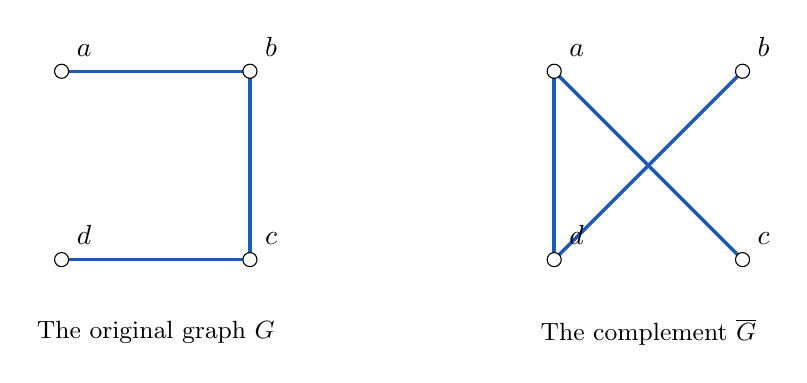
\begin{tikzpicture}[scale=0.92]
			\begin{scope}[xshift=-3.4cm]
				\coordinate (a) at (-1.3,1.3);
				\coordinate (b) at (1.3,1.3);
				\coordinate (c) at (1.3,-1.3);
				\coordinate (d) at (-1.3,-1.3);
				\draw[edge] (a)--(b);
				\draw[edge] (b)--(c);
				\draw[edge] (c)--(d);
				\node[v,label=above right:$a$] at (a) {};
				\node[v,label=above right:$b$] at (b) {};
				\node[v,label=above right:$c$] at (c) {};
				\node[v,label=above right:$d$] at (d) {};
				\node[font=\small,align=center] at (0,-2.3) {The original graph $G$};
			\end{scope}
			\begin{scope}[xshift=3.4cm]
				\coordinate (a) at (-1.3,1.3);
				\coordinate (b) at (1.3,1.3);
				\coordinate (c) at (1.3,-1.3);
				\coordinate (d) at (-1.3,-1.3);
				\draw[edge] (a)--(c);
				\draw[edge] (a)--(d);
				\draw[edge] (b)--(d);
				\node[v,label=above right:$a$] at (a) {};
				\node[v,label=above right:$b$] at (b) {};
				\node[v,label=above right:$c$] at (c) {};
				\node[v,label=above right:$d$] at (d) {};
				\node[font=\small,align=center] at (0,-2.3) {The complement $\overline{G}$};
			\end{scope}
		\end{tikzpicture}
	\end{frame}
	
	\begin{frame}{Special Types of Graphs}
		\begin{block}{Regular graphs}
			A graph is regular if every vertex has the same degree. It is $r$-regular if $\deg(v)=r$ for every vertex $v$.
		\end{block}
		\vspace{0.2cm}\centering
		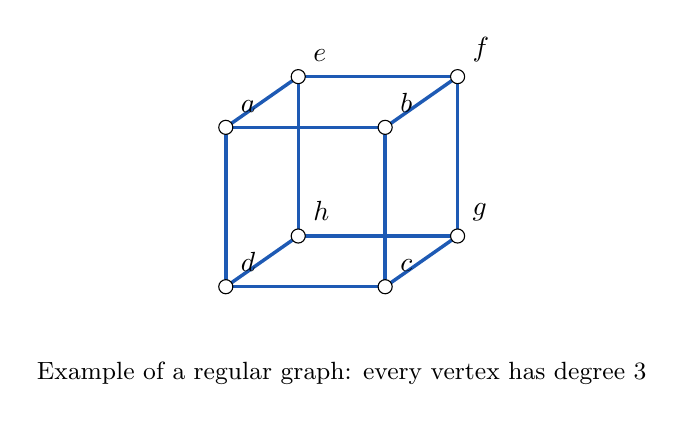
\begin{tikzpicture}[scale=0.92]
			\begin{scope}[xshift=0cm]
				\coordinate (a) at (-1.6,1.1);
				\coordinate (b) at (0.6,1.1);
				\coordinate (c) at (0.6,-1.1);
				\coordinate (d) at (-1.6,-1.1);
				\coordinate (e) at (-0.6,1.8);
				\coordinate (f) at (1.6,1.8);
				\coordinate (g) at (1.6,-0.4);
				\coordinate (h) at (-0.6,-0.4);
				\draw[edge] (a)--(b);
				\draw[edge] (b)--(c);
				\draw[edge] (c)--(d);
				\draw[edge] (d)--(a);
				\draw[edge] (e)--(f);
				\draw[edge] (f)--(g);
				\draw[edge] (g)--(h);
				\draw[edge] (h)--(e);
				\draw[edge] (a)--(e);
				\draw[edge] (b)--(f);
				\draw[edge] (c)--(g);
				\draw[edge] (d)--(h);
				\node[v,label=above right:$a$] at (a) {};
				\node[v,label=above right:$b$] at (b) {};
				\node[v,label=above right:$c$] at (c) {};
				\node[v,label=above right:$d$] at (d) {};
				\node[v,label=above right:$e$] at (e) {};
				\node[v,label=above right:$f$] at (f) {};
				\node[v,label=above right:$g$] at (g) {};
				\node[v,label=above right:$h$] at (h) {};
				\node[font=\small,align=center] at (0,-2.3) {Example of a regular graph: every vertex has degree $3$};
			\end{scope}
		\end{tikzpicture}
	\end{frame}
	
	\begin{frame}{Special Types of Graphs}
		\begin{block}{Cycles}
			The cycle graph $C_n$, for $n\geq 3$, consists of a cycle on $n$ vertices. It has $n$ edges.
		\end{block}
		\vspace{0.2cm}\centering
		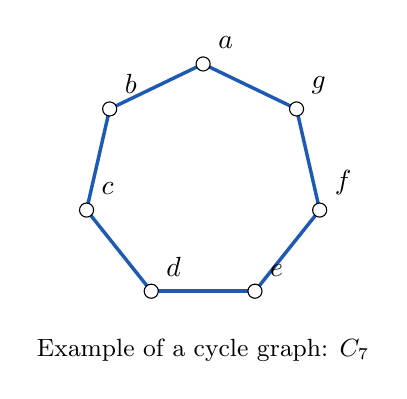
\begin{tikzpicture}[scale=0.92]
			\begin{scope}[xshift=0cm]
				\coordinate (a) at (0.0,1.65);
				\coordinate (b) at (-1.29,1.029);
				\coordinate (c) at (-1.609,-0.367);
				\coordinate (d) at (-0.716,-1.487);
				\coordinate (e) at (0.716,-1.487);
				\coordinate (f) at (1.609,-0.367);
				\coordinate (g) at (1.29,1.029);
				\draw[edge] (a)--(b);
				\draw[edge] (b)--(c);
				\draw[edge] (c)--(d);
				\draw[edge] (d)--(e);
				\draw[edge] (e)--(f);
				\draw[edge] (f)--(g);
				\draw[edge] (g)--(a);
				\node[v,label=above right:$a$] at (a) {};
				\node[v,label=above right:$b$] at (b) {};
				\node[v,label=above right:$c$] at (c) {};
				\node[v,label=above right:$d$] at (d) {};
				\node[v,label=above right:$e$] at (e) {};
				\node[v,label=above right:$f$] at (f) {};
				\node[v,label=above right:$g$] at (g) {};
				\node[font=\small,align=center] at (0,-2.3) {Example of a cycle graph: $C_7$};
			\end{scope}
		\end{tikzpicture}
	\end{frame}
	
	\begin{frame}{Special Types of Graphs}
		\begin{block}{Paths}
			The path graph $P_n$ consists of a path on $n$ vertices. It has $n-1$ edges.
		\end{block}
		\vspace{0.2cm}\centering
		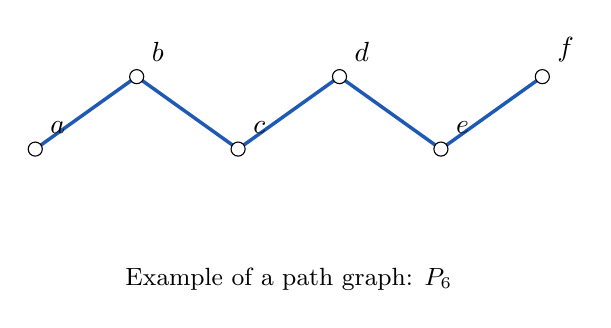
\begin{tikzpicture}[scale=0.92]
			\begin{scope}[xshift=0cm]
				\coordinate (a) at (-3.5,-0.5);
				\coordinate (b) at (-2.1,0.5);
				\coordinate (c) at (-0.7000000000000002,-0.5);
				\coordinate (d) at (0.6999999999999993,0.5);
				\coordinate (e) at (2.0999999999999996,-0.5);
				\coordinate (f) at (3.5,0.5);
				\draw[edge] (a)--(b);
				\draw[edge] (b)--(c);
				\draw[edge] (c)--(d);
				\draw[edge] (d)--(e);
				\draw[edge] (e)--(f);
				\node[v,label=above right:$a$] at (a) {};
				\node[v,label=above right:$b$] at (b) {};
				\node[v,label=above right:$c$] at (c) {};
				\node[v,label=above right:$d$] at (d) {};
				\node[v,label=above right:$e$] at (e) {};
				\node[v,label=above right:$f$] at (f) {};
				\node[font=\small,align=center] at (0,-2.3) {Example of a path graph: $P_6$};
			\end{scope}
		\end{tikzpicture}
	\end{frame}
	
	\begin{frame}{Special Types of Graphs}
		\begin{block}{Subgraphs}
			A graph $H$ is a subgraph of $G$ if $V(H)\subseteq V(G)$ and $E(H)\subseteq E(G)$. We write $H\subseteq G$.
		\end{block}
		\vspace{0.2cm}\centering
		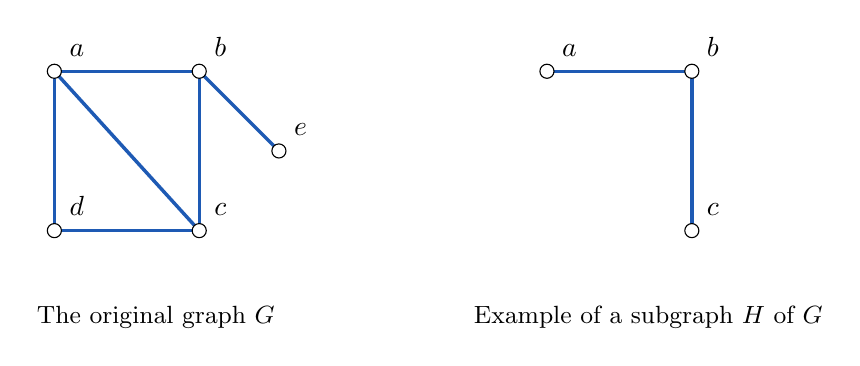
\begin{tikzpicture}[scale=0.92]
			\begin{scope}[xshift=-3.4cm]
				\coordinate (a) at (-1.4,1.1);
				\coordinate (b) at (0.6,1.1);
				\coordinate (c) at (0.6,-1.1);
				\coordinate (d) at (-1.4,-1.1);
				\coordinate (e) at (1.7,0);
				\draw[edge] (a)--(b);
				\draw[edge] (b)--(c);
				\draw[edge] (c)--(d);
				\draw[edge] (d)--(a);
				\draw[edge] (a)--(c);
				\draw[edge] (b)--(e);
				\node[v,label=above right:$a$] at (a) {};
				\node[v,label=above right:$b$] at (b) {};
				\node[v,label=above right:$c$] at (c) {};
				\node[v,label=above right:$d$] at (d) {};
				\node[v,label=above right:$e$] at (e) {};
				\node[font=\small,align=center] at (0,-2.3) {The original graph $G$};
			\end{scope}
			\begin{scope}[xshift=3.4cm]
				\coordinate (a) at (-1.4,1.1);
				\coordinate (b) at (0.6,1.1);
				\coordinate (c) at (0.6,-1.1);
				\draw[edge] (a)--(b);
				\draw[edge] (b)--(c);
				\node[v,label=above right:$a$] at (a) {};
				\node[v,label=above right:$b$] at (b) {};
				\node[v,label=above right:$c$] at (c) {};
				\node[font=\small,align=center] at (0,-2.3) {Example of a subgraph $H$ of $G$};
			\end{scope}
		\end{tikzpicture}
	\end{frame}
	
	\begin{frame}{Special Types of Graphs}
		\begin{block}{Induced subgraphs}
			For $S\subseteq V(G)$, the induced subgraph $G[S]$ has vertex set $S$ and includes every edge of $G$ with both end vertices in $S$.
		\end{block}
		\vspace{0.2cm}\centering
		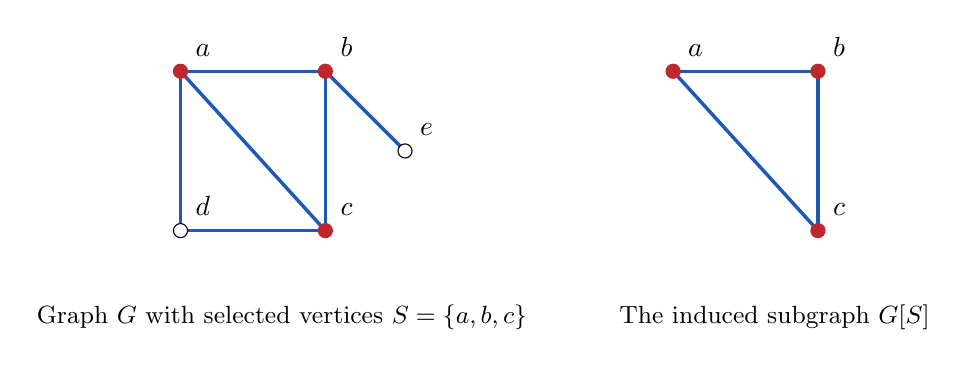
\begin{tikzpicture}[scale=0.92]
			\begin{scope}[xshift=-3.4cm]
				\coordinate (a) at (-1.4,1.1);
				\coordinate (b) at (0.6,1.1);
				\coordinate (c) at (0.6,-1.1);
				\coordinate (d) at (-1.4,-1.1);
				\coordinate (e) at (1.7,0);
				\draw[edge] (a)--(b);
				\draw[edge] (b)--(c);
				\draw[edge] (c)--(d);
				\draw[edge] (d)--(a);
				\draw[edge] (a)--(c);
				\draw[edge] (b)--(e);
				\node[v,fill=RamRed,draw=RamRed,label=above right:$a$] at (a) {};
				\node[v,fill=RamRed,draw=RamRed,label=above right:$b$] at (b) {};
				\node[v,fill=RamRed,draw=RamRed,label=above right:$c$] at (c) {};
				\node[v,label=above right:$d$] at (d) {};
				\node[v,label=above right:$e$] at (e) {};
				\node[font=\small,align=center] at (0,-2.3) {Graph $G$ with selected vertices $S=\{a,b,c\}$};
			\end{scope}
			\begin{scope}[xshift=3.4cm]
				\coordinate (a) at (-1.4,1.1);
				\coordinate (b) at (0.6,1.1);
				\coordinate (c) at (0.6,-1.1);
				\draw[edge] (a)--(b);
				\draw[edge] (b)--(c);
				\draw[edge] (a)--(c);
				\node[v,fill=RamRed,draw=RamRed,label=above right:$a$] at (a) {};
				\node[v,fill=RamRed,draw=RamRed,label=above right:$b$] at (b) {};
				\node[v,fill=RamRed,draw=RamRed,label=above right:$c$] at (c) {};
				\node[font=\small,align=center] at (0,-2.3) {The induced subgraph $G[S]$};
			\end{scope}
		\end{tikzpicture}
	\end{frame}
	
	\begin{frame}{Special Types of Graphs: Bipartite Graphs}
		\begin{block}{Bipartite graphs}
			A graph is bipartite if its vertex set can be partitioned into two disjoint sets $X$ and $Y$ such that every edge has one end vertex in $X$ and the other in $Y$. The sets $X$ and $Y$ are called the partite sets.
		\end{block}
		\vspace{0.2cm}
		\centering
		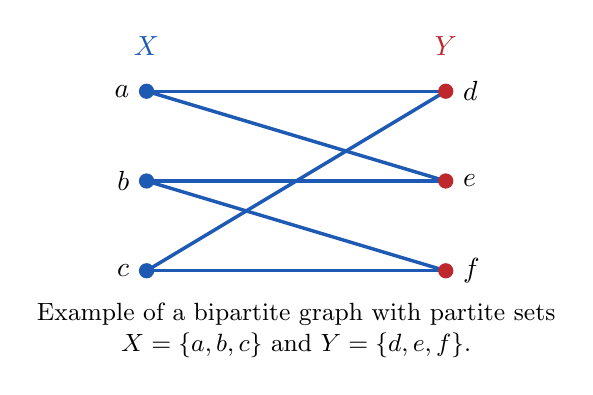
\begin{tikzpicture}[scale=0.95]
			\coordinate (a) at (-2,1.2);
			\coordinate (b) at (-2,0);
			\coordinate (c) at (-2,-1.2);
			\coordinate (d) at (2,1.2);
			\coordinate (e) at (2,0);
			\coordinate (f) at (2,-1.2);
			\foreach \x/\y in {a/d,a/e,b/e,b/f,c/d,c/f}
			\draw[edge] (\x)--(\y);
			\foreach \p in {a,b,c}
			\node[v,fill=RamBlue,draw=RamBlue,label=left:$\p$] at (\p) {};
			\foreach \p in {d,e,f}
			\node[v,fill=RamRed,draw=RamRed,label=right:$\p$] at (\p) {};
			\node[RamBlue] at (-2,1.8) {$X$};
			\node[RamRed] at (2,1.8) {$Y$};
			\node[font=\small,align=center] at (0,-2) {Example of a bipartite graph with partite sets\\$X=\{a,b,c\}$ and $Y=\{d,e,f\}$.};
		\end{tikzpicture}
	\end{frame}
	
	\begin{frame}[t]{Theorem: Bipartite Graphs and Odd Cycles}
		\vspace{0.2cm}
		\begin{block}{Theorem 1.3}
			A graph with at least two vertices is bipartite if and only if it contains no odd cycles.
		\end{block}
	\end{frame}
	
	\begin{frame}[t]{Proof of Theorem}
		\small
		\begin{block}{Theorem 1.3}
			A graph with at least two vertices is bipartite if and only if it contains no odd cycles.
			
		\end{block}
		\begin{block}{Proof: Forward direction}
			Let $G$ be bipartite with partite sets $X$ and $Y$. Along a cycle, successive vertices alternate between $X$ and $Y$. Starting in $X$, we are in $X$ after an even number of edges and in $Y$ after an odd number. Returning to the starting vertex therefore requires an even number of edges.
		\end{block}
		\vspace{0.1cm}
		\centering
		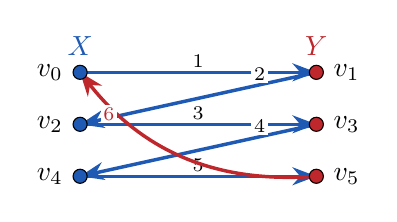
\begin{tikzpicture}[scale=0.6]
			\coordinate (a) at (-2.5,1.1);
			\coordinate (c) at (-2.5,0);
			\coordinate (e) at (-2.5,-1.1);
			\coordinate (b) at (2.5,1.1);
			\coordinate (d) at (2.5,0);
			\coordinate (f) at (2.5,-1.1);
			\foreach \u/\v/\num in {a/b/1,c/d/3,e/f/5}
			\draw[edge,-{Stealth}] (\u)--node[above,font=\scriptsize,fill=white,inner sep=1pt] {$\num$} (\v);
			\draw[edge,-{Stealth}] (b)--node[pos=0.24,above,font=\scriptsize,fill=white,inner sep=1pt] {$2$} (c);
			\draw[edge,-{Stealth}] (d)--node[pos=0.24,above,font=\scriptsize,fill=white,inner sep=1pt] {$4$} (e);
			\draw[RamRed,line width=1.25pt,-{Stealth}] (f) to[bend left=28] node[pos=0.8,left,font=\scriptsize,fill=white,inner sep=1pt] {$6$} (a);
			\foreach \p/\lab in {a/v_0,c/v_2,e/v_4}
			\node[v,fill=RamBlue,label=left:$\lab$] at (\p) {};
			\foreach \p/\lab in {b/v_1,d/v_3,f/v_5}
			\node[v,fill=RamRed,label=right:$\lab$] at (\p) {};
			\node[RamBlue] at (-2.5,1.65) {$X$};
			\node[RamRed] at (2.5,1.65) {$Y$};
		\end{tikzpicture}
		\par\vspace{0.05cm}
		{\small Each step switches sides. Hence, you will need to do an even number of steps to return to the same side. In particular, you will need to do an even number of steps to return to the same vertex.}
	\end{frame}
	
	\begin{frame}[t]{Proof of Theorem}
		\small
		\begin{block}{Theorem 1.3}
			A graph with at least two vertices is bipartite if and only if it contains no odd cycles.
		\end{block}
		\begin{block}{Proof: Reverse direction}
			\footnotesize
			Suppose $G$ has no odd cycles. We may assume $G$ is connected, treating each connected component separately otherwise. Fix a vertex $v$ and define
			\[
			X=\{u\in V(G):d(v,u)\text{ is even}\},\qquad
			Y=\{u\in V(G):d(v,u)\text{ is odd}\}.
			\]
			Here $d(v,u)$ is the length of a shortest path from $v$ to $u$.
			
			\medskip
			It suffices to show that no two vertices in $X$ are adjacent, and similarly for $Y$. Since $X$ and $Y$ partition $V(G)$, every edge must then have exactly one end vertex in each set. Thus $G$ is bipartite.
		\end{block}
		\centering
		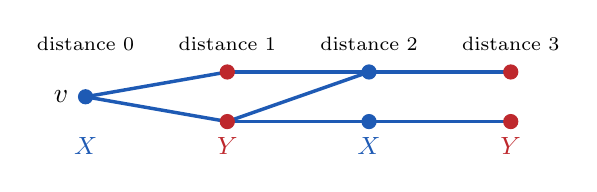
\begin{tikzpicture}[x=1.8cm,y=0.45cm]
			\coordinate (x) at (0,0);
			\coordinate (a) at (1,0.7); \coordinate (b) at (1,-0.7);
			\coordinate (c) at (2,0.7); \coordinate (d) at (2,-0.7);
			\coordinate (e) at (3,0.7); \coordinate (f) at (3,-0.7);
			\foreach \u/\v in {x/a,x/b,a/c,b/c,b/d,c/e,d/f}
			\draw[edge] (\u)--(\v);
			\node[v,fill=RamBlue,draw=RamBlue,label=left:$v$] at (x) {};
			\foreach \p in {c,d} \node[v,fill=RamBlue,draw=RamBlue] at (\p) {};
			\foreach \p in {a,b,e,f} \node[v,fill=RamRed,draw=RamRed] at (\p) {};
			\foreach \i in {0,1,2,3} \node[font=\scriptsize] at (\i,1.5) {distance $\i$};
			\foreach \i in {0,2} \node[RamBlue,font=\small] at (\i,-1.4) {$X$};
			\foreach \i in {1,3} \node[RamRed,font=\small] at (\i,-1.4) {$Y$};
		\end{tikzpicture}
		
	\end{frame}
	
	\begin{frame}[t]{Proof of Theorem}
		\small
		\begin{block}{Theorem 1.3}
			A graph with at least two vertices is bipartite if and only if it contains no odd cycles.
		\end{block}
		\begin{block}{Proof: Reverse direction continued}
			\footnotesize
			We argue by contradiction. Suppose $x,x'\in X$ are adjacent. Choose shortest paths from $v$ to $x$ and from $v$ to $x'$, of lengths $2r$ and $2s$. Let $z$ be their last common vertex and put $t=d(v,z)$.
			
			\medskip
			The portions from $z$ to $x$ and $x'$ meet only at $z$. Together with $xx'$, they form a cycle of length
			\[
			(2r-t)+(2s-t)+1=2(r+s-t)+1,
			\]
			which is odd, a contradiction. The same argument applies to two vertices in $Y$.
		\end{block}
		\centering
		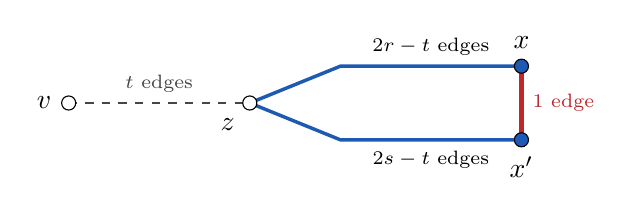
\begin{tikzpicture}[x=1.15cm,y=0.55cm]
			\coordinate (v) at (-3,0);
			\coordinate (z) at (-1,0);
			\coordinate (a) at (0,0.85);
			\coordinate (b) at (0,-0.85);
			\coordinate (x) at (2,0.85);
			\coordinate (xx) at (2,-0.85);
			\draw[DarkGray,line width=1pt,dashed] (v)--node[above,font=\scriptsize] {$t$ edges} (z);
			\draw[edge] (z)--(a)--node[above,font=\scriptsize] {$2r-t$ edges} (x);
			\draw[edge] (z)--(b)--node[below,font=\scriptsize] {$2s-t$ edges} (xx);
			\draw[RamRed,line width=1.5pt] (x)--node[right,font=\scriptsize] {$1$ edge} (xx);
			\node[v,label=left:$v$] at (v) {};
			\node[v,label=below left:$z$] at (z) {};
			\node[v,fill=RamBlue,label=above:$x$] at (x) {};
			\node[v,fill=RamBlue,label=below:$x'$] at (xx) {};
		\end{tikzpicture}
		
	\end{frame}
	
	\begin{frame}{Graph Isomorphisms}
		\centering
		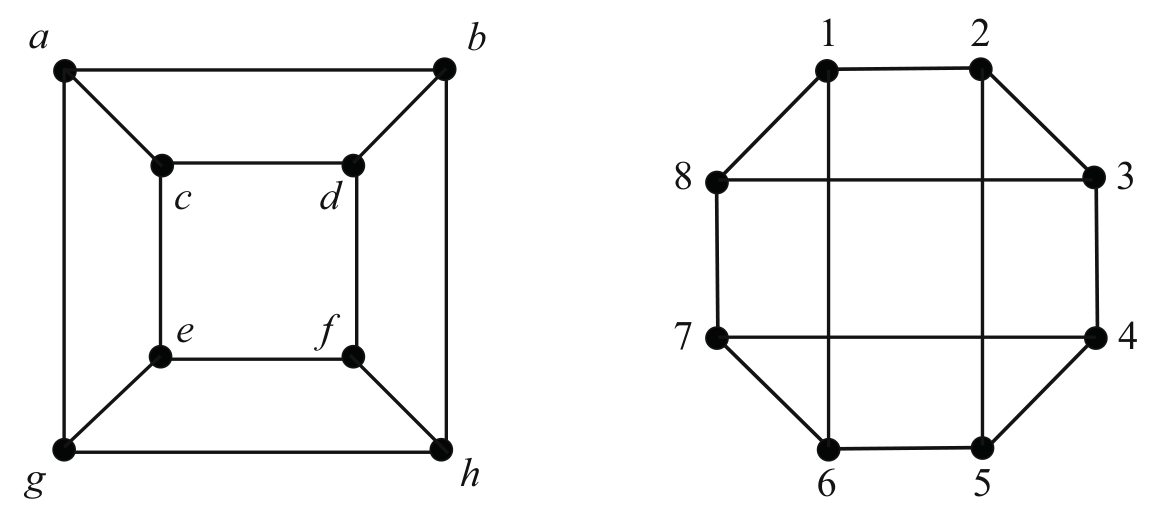
\includegraphics[width=0.82\textwidth]{figure_1_21_graphs.png}
		\par\vspace{0.4cm}
		{\Large\color{RamBlue}Are these graphs the same?}
		\par\vspace{0.35cm}
		{\scriptsize Source: Harris, Hirst, and Mossinghoff, \textit{Combinatorics and Graph Theory}, 2nd ed., Figure 1.21.}
	\end{frame}
	
	\begin{frame}{Are the Graphs the Same: Yes}
		\centering
		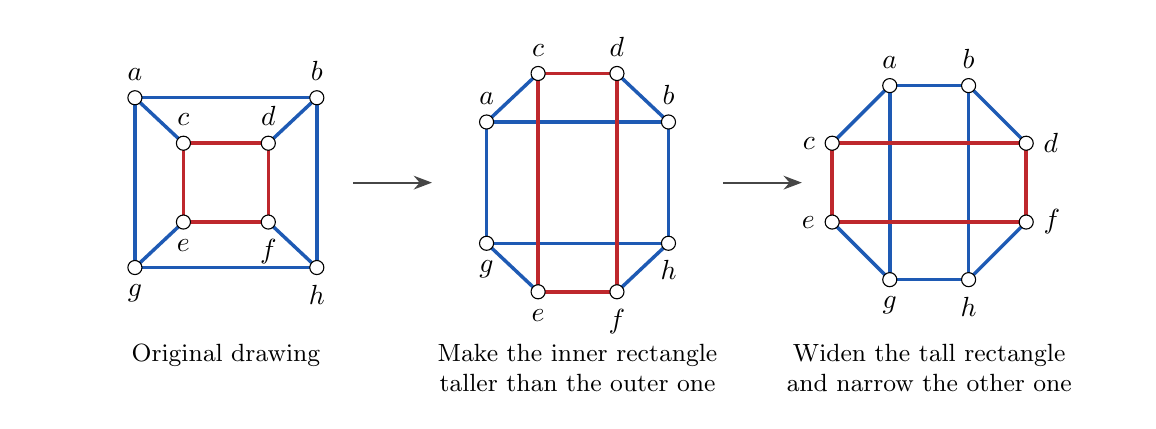
\begin{tikzpicture}[scale=0.77]
			\begin{scope}[xshift=-5.8cm]
				\coordinate (a) at (-1.5,1.4);
				\coordinate (b) at (1.5,1.4);
				\coordinate (c) at (-0.7,0.65);
				\coordinate (d) at (0.7,0.65);
				\coordinate (e) at (-0.7,-0.65);
				\coordinate (f) at (0.7,-0.65);
				\coordinate (g) at (-1.5,-1.4);
				\coordinate (h) at (1.5,-1.4);
				\draw[edge] (a)--(b);
				\draw[edge] (b)--(h);
				\draw[edge] (h)--(g);
				\draw[edge] (g)--(a);
				\draw[edge] (a)--(c);
				\draw[edge] (b)--(d);
				\draw[edge] (g)--(e);
				\draw[edge] (h)--(f);
				\draw[RamRed,line width=1.25pt] (c)--(d);
				\draw[RamRed,line width=1.25pt] (d)--(f);
				\draw[RamRed,line width=1.25pt] (f)--(e);
				\draw[RamRed,line width=1.25pt] (e)--(c);
				\node[v,label=above:$a$] at (a) {};
				\node[v,label=above:$b$] at (b) {};
				\node[v,label=above:$c$] at (c) {};
				\node[v,label=above:$d$] at (d) {};
				\node[v,label=below:$e$] at (e) {};
				\node[v,label=below:$f$] at (f) {};
				\node[v,label=below:$g$] at (g) {};
				\node[v,label=below:$h$] at (h) {};
				\node[font=\small,align=center,anchor=north,text width=4.8cm] at (0,-2.5) {Original drawing};
			\end{scope}
			\begin{scope}[xshift=0.0cm]
				\coordinate (a) at (-1.5,1);
				\coordinate (b) at (1.5,1);
				\coordinate (c) at (-0.65,1.8);
				\coordinate (d) at (0.65,1.8);
				\coordinate (e) at (-0.65,-1.8);
				\coordinate (f) at (0.65,-1.8);
				\coordinate (g) at (-1.5,-1);
				\coordinate (h) at (1.5,-1);
				\draw[edge] (a)--(b);
				\draw[edge] (b)--(h);
				\draw[edge] (h)--(g);
				\draw[edge] (g)--(a);
				\draw[edge] (a)--(c);
				\draw[edge] (b)--(d);
				\draw[edge] (g)--(e);
				\draw[edge] (h)--(f);
				\draw[RamRed,line width=1.25pt] (c)--(d);
				\draw[RamRed,line width=1.25pt] (d)--(f);
				\draw[RamRed,line width=1.25pt] (f)--(e);
				\draw[RamRed,line width=1.25pt] (e)--(c);
				\node[v,label=above:$a$] at (a) {};
				\node[v,label=above:$b$] at (b) {};
				\node[v,label=above:$c$] at (c) {};
				\node[v,label=above:$d$] at (d) {};
				\node[v,label=below:$e$] at (e) {};
				\node[v,label=below:$f$] at (f) {};
				\node[v,label=below:$g$] at (g) {};
				\node[v,label=below:$h$] at (h) {};
				\node[font=\small,align=center,anchor=north,text width=4.8cm] at (0,-2.5) {Make the inner rectangle\\taller than the outer one};
			\end{scope}
			\begin{scope}[xshift=5.8cm]
				\coordinate (a) at (-0.65,1.6);
				\coordinate (b) at (0.65,1.6);
				\coordinate (c) at (-1.6,0.65);
				\coordinate (d) at (1.6,0.65);
				\coordinate (e) at (-1.6,-0.65);
				\coordinate (f) at (1.6,-0.65);
				\coordinate (g) at (-0.65,-1.6);
				\coordinate (h) at (0.65,-1.6);
				\draw[edge] (a)--(b);
				\draw[edge] (b)--(h);
				\draw[edge] (h)--(g);
				\draw[edge] (g)--(a);
				\draw[edge] (a)--(c);
				\draw[edge] (b)--(d);
				\draw[edge] (g)--(e);
				\draw[edge] (h)--(f);
				\draw[RamRed,line width=1.25pt] (c)--(d);
				\draw[RamRed,line width=1.25pt] (d)--(f);
				\draw[RamRed,line width=1.25pt] (f)--(e);
				\draw[RamRed,line width=1.25pt] (e)--(c);
				\node[v,label=above:$a$] at (a) {};
				\node[v,label=above:$b$] at (b) {};
				\node[v,label=left:$c$] at (c) {};
				\node[v,label=right:$d$] at (d) {};
				\node[v,label=left:$e$] at (e) {};
				\node[v,label=right:$f$] at (f) {};
				\node[v,label=below:$g$] at (g) {};
				\node[v,label=below:$h$] at (h) {};
				\node[font=\small,align=center,anchor=north,text width=4.8cm] at (0,-2.5) {Widen the tall rectangle\\and narrow the other one};
			\end{scope}
			\draw[-{Stealth},thick,DarkGray] (-3.7,0)--(-2.4,0);
			\draw[-{Stealth},thick,DarkGray] (2.4,0)--(3.7,0);
		\end{tikzpicture}
		\par\vspace{0.3cm}
		Every edge keeps the same end vertices throughout.
		\par\vspace{0.25cm}
		{\small To match the book's labels: $a\mapsto1$, $b\mapsto2$, $c\mapsto8$, $d\mapsto3$,\\
			$e\mapsto7$, $f\mapsto4$, $g\mapsto6$, $h\mapsto5$.}
	\end{frame}
	
	\begin{frame}{Definition: Graph Isomorphism}
		\begin{block}{Graph isomorphism}
			Graphs $G$ and $H$ are \textbf{isomorphic} if there exists a one-to-one correspondence
			\[
			f:V(G)\longrightarrow V(H)
			\]
			such that, for every pair of vertices $x,y\in V(G)$,
			\[
			xy\in E(G)\quad\Longleftrightarrow\quad f(x)f(y)\in E(H).
			\]
			The mapping $f$ is called an \textbf{isomorphism}.
		\end{block}
		\vspace{0.25cm}
		\textbf{\color{RamBlue}Example:} For the two graphs on the previous slides, an isomorphism is
		\[
		\begin{array}{c|cccccccc}
			x & a & b & c & d & e & f & g & h\\ \hline
			f(x) & 1 & 2 & 8 & 3 & 7 & 4 & 6 & 5
		\end{array}
		\]
		For example, the edge $ac$ corresponds to the edge $18$.
	\end{frame}
	
	\begin{frame}{Graph Isomorphisms Continued}
		\begin{block}{Properties preserved by an isomorphism}
			If $G$ and $H$ are isomorphic, then they have:
			\begin{itemize}
				\item The same number of vertices and the same number of edges.
				\item The same degree at corresponding vertices, hence identical degree sequences.
				\item The same connectivity and the same numbers of cycles of each length.
			\end{itemize}
			Their complements $\overline{G}$ and $\overline{H}$ are also isomorphic, using the same vertex correspondence.
		\end{block}
		\vspace{0.2cm}
		Matching vertex counts, edge counts, and degree sequences alone does not guarantee that two graphs are isomorphic.
		
		\medskip
		In general, determining whether two graphs are isomorphic can be difficult, especially as the graphs become large.
	\end{frame}
	
	\begin{frame}[plain]
		\centering
		{\LARGE\color{RamBlue}Next time: Distance in Graphs}
	\end{frame}
	
\end{document}
